\documentclass[12pt,a4paper]{article}

\usepackage{graphicx}
\usepackage[hidelinks,hypertexnames=false]{hyperref}
\usepackage{geometry}
\usepackage{array}
\usepackage{float}
\usepackage{amsmath,amssymb,amsfonts}
\usepackage{booktabs}
\usepackage{microtype}

\geometry{margin=2.5cm}

\title{Supplementary Material: A Hierarchical Virtual-Pursuit-Point Maneuver Interface for Close-Range Air Combat}
\author{}
\date{}

\begin{document}

\renewcommand{\thetable}{S\arabic{table}}
\renewcommand{\thefigure}{S\arabic{figure}}

\maketitle

\section{Supplementary Tables}

\subsection{Table S1: Evaluation outcome summary}

Table~\ref{tab:evaluation_outcomes} reports the evaluation outcome summary by opponent and task for both the oracle static gate and the learned PPO high-level policy, including the 95\% Wilson score confidence interval for each proportion. These values match the main-text outcome table exactly.

\begin{table}[htbp]
\centering
\caption{Evaluation outcomes by opponent and task (aggregate summary).}
\label{tab:evaluation_outcomes}
\resizebox{\textwidth}{!}{%
\begin{tabular}{@{}llcccccc@{}}
\toprule
Opponent & Task & Method & $N_{\text{total}}$ & $N_{\text{resolved}}$ & Wins & Losses & Win Rate (95\% Wilson CI) \\
\midrule
expert & head\_on & Oracle & 60 & 60 & 34 & 26 & 0.5667 [0.4410, 0.6843] \\
expert & head\_on & PPO & 60 & 60 & 39 & 21 & 0.6500 [0.5236, 0.7583] \\
expert & crossing\_feasible & Oracle & 4 & 4 & 3 & 1 & 0.7500 [0.3006, 0.9544] \\
expert & crossing\_feasible & PPO & 4 & 4 & 3 & 1 & 0.7500 [0.3006, 0.9544] \\
end\_to\_end & head\_on & Oracle & 60 & 59 & 55 & 4 & 0.9322 [0.8382, 0.9733] \\
end\_to\_end & head\_on & PPO & 60 & 60 & 54 & 6 & 0.9000 [0.7985, 0.9534] \\
end\_to\_end & crossing\_feasible & Oracle & 4 & 4 & 3 & 1 & 0.7500 [0.3006, 0.9544] \\
end\_to\_end & crossing\_feasible & PPO & 4 & 4 & 3 & 1 & 0.7500 [0.3006, 0.9544] \\
\bottomrule
\end{tabular}
}
\end{table}

\subsection{Table S2: Representative excerpts for expert head-on, post-repair policy}

Table~\ref{tab:scenario_breakdown} lists representative individual scenario outcomes for the post-repair policy on the expert/head\_on split. The full per-scenario table is archived in the reproduction bundle.

\begin{table}[htbp]
\centering
\caption{Representative per-scenario excerpts for expert/head\_on, post-repair policy.}
\label{tab:scenario_breakdown}
\begin{tabular}{@{}>{\raggedright\arraybackslash}p{7.5cm}ccc@{}}
\toprule
Scenario & Outcome & Steps & Time (s) \\
\midrule
\url{head_on_manifest_r1600_v195_v195_alt0} & Win & 3500 & 29.2 \\
\url{head_on_manifest_r3300_v245_v255_altm450} & Win & 4800 & 40.0 \\
\url{head_on_manifest_r2000_v200_v200_altm200_yneg150} & Loss & 2800 & 23.3 \\
\bottomrule
\end{tabular}
\end{table}

\subsection{Table S3 and Figure S3: Crossing Evidence Synthesis}

Table~\ref{tab:crossing_evidence_synthesis} brings together the legacy G4
counterexample, the preregistered 24-scenario independent RQ1 crossing
envelope, and the three independently trained PPO seeds. The primary contrast
is the paired resolved win-rate difference between PPO high-level routing and
the fixed head-on VPP reference. The static oracle is reported in the source
data as a privileged task-label reference and is not treated as a symmetric
learned-policy comparator. The G4 row is retained because it is a genuine
counterexample in the earlier four-scenario scope; it is not omitted after the
larger RQ1 envelope was introduced.

\noindent\textit{Numerical provenance.} The authoritative source identifiers,
clean-run directory names, and claim boundaries are listed in the accompanying
authoritative artifact index. The RQ1 rows are
supporting finite-envelope preservation evidence and are not pooled with the
canonical dual-opponent headline results in Table~\ref{tab:evaluation_outcomes}.

\begin{table*}[htbp]
\centering
\caption{Crossing evidence synthesis. Wilson intervals describe each method's
resolved win proportion; paired bootstrap intervals describe PPO-minus-fixed
differences using scenario-pair resampling (100,000 deterministic resamples).
The $-0.05$ threshold is a preregistered practical preservation screen, not a
test of statistical superiority. The final two rows summarize three PPO policy
seeds as mean $\pm$ population standard deviation; they are descriptive and
have no pooled bootstrap interval.}
\label{tab:crossing_evidence_synthesis}
\scriptsize
\resizebox{\textwidth}{!}{%
\begin{tabular}{@{}lllrrrll@{}}
\toprule
Evidence & Opponent & PPO seed & $N$ & PPO wins & Fixed wins & PPO Wilson / Fixed Wilson & Paired $\Delta$ [95\% bootstrap] \\
\midrule
G4 legacy check & end-to-end & canonical & 4 & 3 & 4 & 0.750 [0.301, 0.954] / 1.000 [0.510, 1.000] & -0.250 [-0.750, 0.000] \\
RQ1 independent envelope & expert & canonical & 24 & 11 & 8 & 0.458 [0.279, 0.649] / 0.333 [0.180, 0.533] & +0.125 [-0.042, 0.292] \\
RQ1 independent envelope & end-to-end & canonical & 24 & 18 & 19 & 0.750 [0.551, 0.880] / 0.792 [0.595, 0.908] & -0.042 [-0.167, 0.083] \\
RQ1 seed robustness & expert & 701 & 24 & 12 & 8 & 0.500 [0.314, 0.686] / 0.333 [0.180, 0.533] & +0.167 [-0.042, 0.375] \\
RQ1 seed robustness & expert & 702 & 24 & 7 & 8 & 0.292 [0.149, 0.492] / 0.333 [0.180, 0.533] & -0.042 [-0.250, 0.167] \\
RQ1 seed robustness & expert & 703 & 24 & 7 & 8 & 0.292 [0.149, 0.492] / 0.333 [0.180, 0.533] & -0.042 [-0.250, 0.167] \\
RQ1 seed robustness & end-to-end & 701 & 24 & 19 & 19 & 0.792 [0.595, 0.908] / 0.792 [0.595, 0.908] & +0.000 [-0.125, 0.125] \\
RQ1 seed robustness & end-to-end & 702 & 24 & 19 & 19 & 0.792 [0.595, 0.908] / 0.792 [0.595, 0.908] & +0.000 [-0.125, 0.125] \\
RQ1 seed robustness & end-to-end & 703 & 24 & 19 & 19 & 0.792 [0.595, 0.908] / 0.792 [0.595, 0.908] & +0.000 [-0.125, 0.125] \\
\midrule
Across clean-import seeds & expert & 701--703 & $3\!\times\!24$ & -- & -- & 0.361 $\pm$ 0.098 / 0.333 $\pm$ 0.000 & +0.028 $\pm$ 0.098 \\
Across clean-import seeds & end-to-end & 701--703 & $3\!\times\!24$ & -- & -- & 0.792 $\pm$ 0.000 / 0.792 $\pm$ 0.000 & +0.000 $\pm$ 0.000 \\
\bottomrule
\end{tabular}
}
\end{table*}

The two canonical RQ1 rows meet the $-0.05$ preservation screen under both
opponents. All six seed-by-opponent cells also meet it; however, expert PPO
win rates range from 0.292 to 0.500 (mean $0.361$, population standard
deviation $0.098$); the corresponding mean paired gap is $+0.028 \pm 0.098$.
End-to-end PPO rates and paired gaps are $0.792 \pm 0.000$ and $+0.000 \pm
0.000$, respectively. Thus the seed study supports threshold robustness, not
invariant routing behavior or superiority. A direct-script training attempt
that imported an exploratory source tree through an ambient Python path was
invalidated before evaluation; only the three clean-import cohort checkpoints
in Table~\ref{tab:crossing_evidence_synthesis} are included.
Terminal-event decompositions, raw paired outcomes, checkpoint hashes, and
run manifests are machine-readable in the reproduction bundle.

\section{Supplementary Figures}

\subsection{Figure S1: Residual diagnostic top-down view}

\begin{figure}[htbp]
\centering
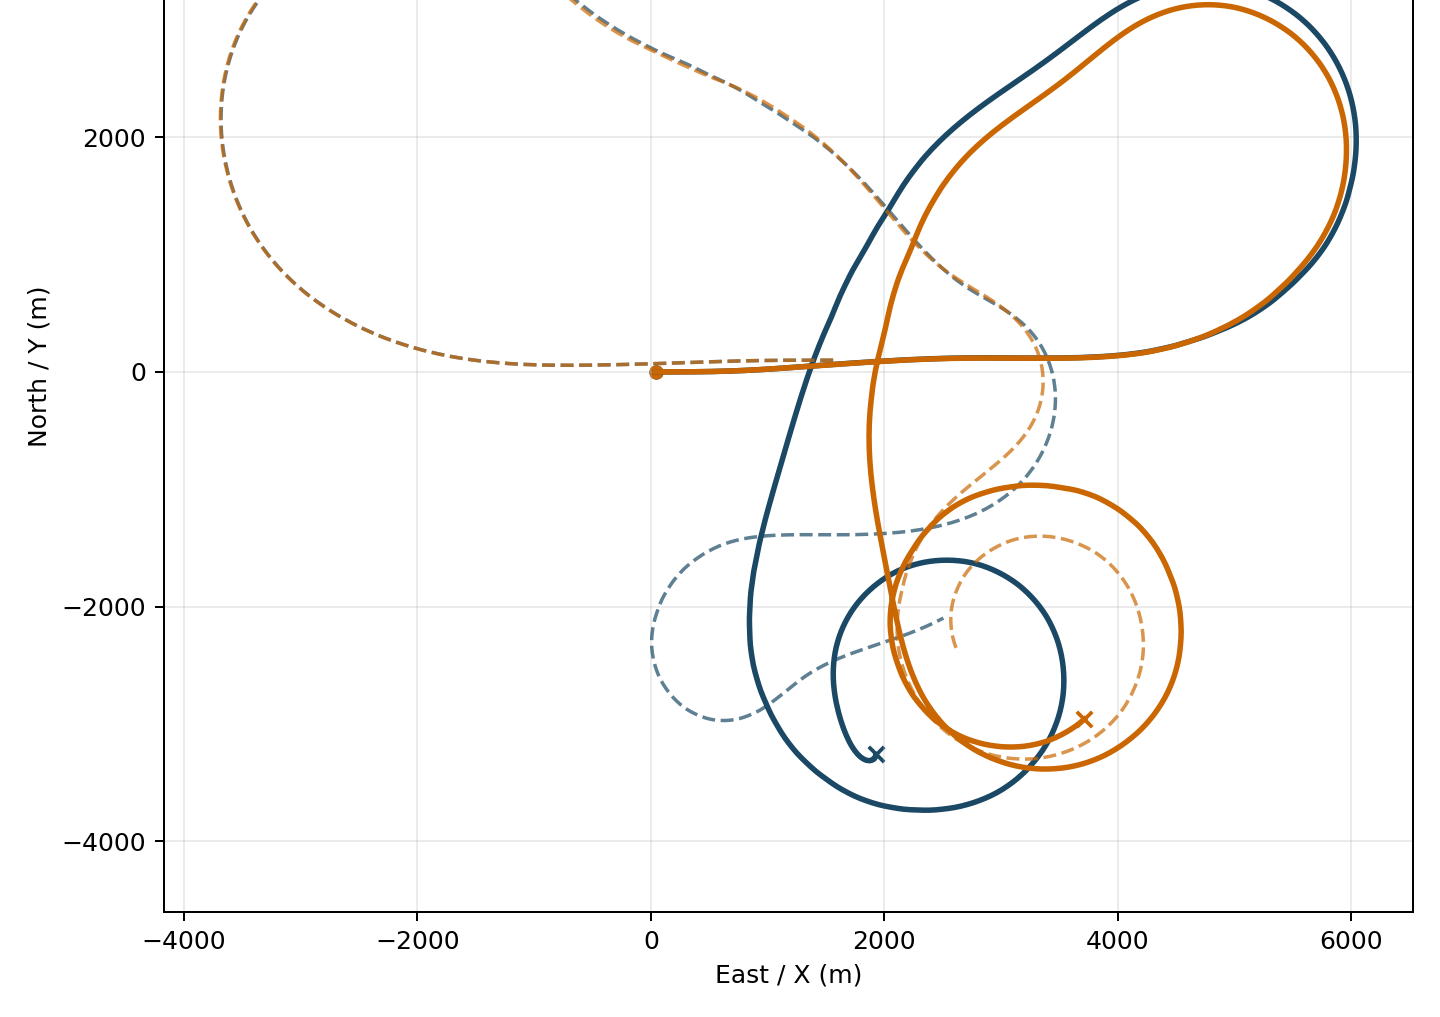
\includegraphics[width=0.85\textwidth]{figures_ast/fig1_formal_residual_r1600_topdown_oracle_vs_recovery.png}
\caption{Residual diagnostic: expert/head\_on top-down trajectory comparison. Oracle static gate (blue) vs. post-repair policy (orange).}
\label{fig:s1}
\end{figure}

\subsection{Figure S2: Residual diagnostic time series}

\begin{figure}[htbp]
\centering
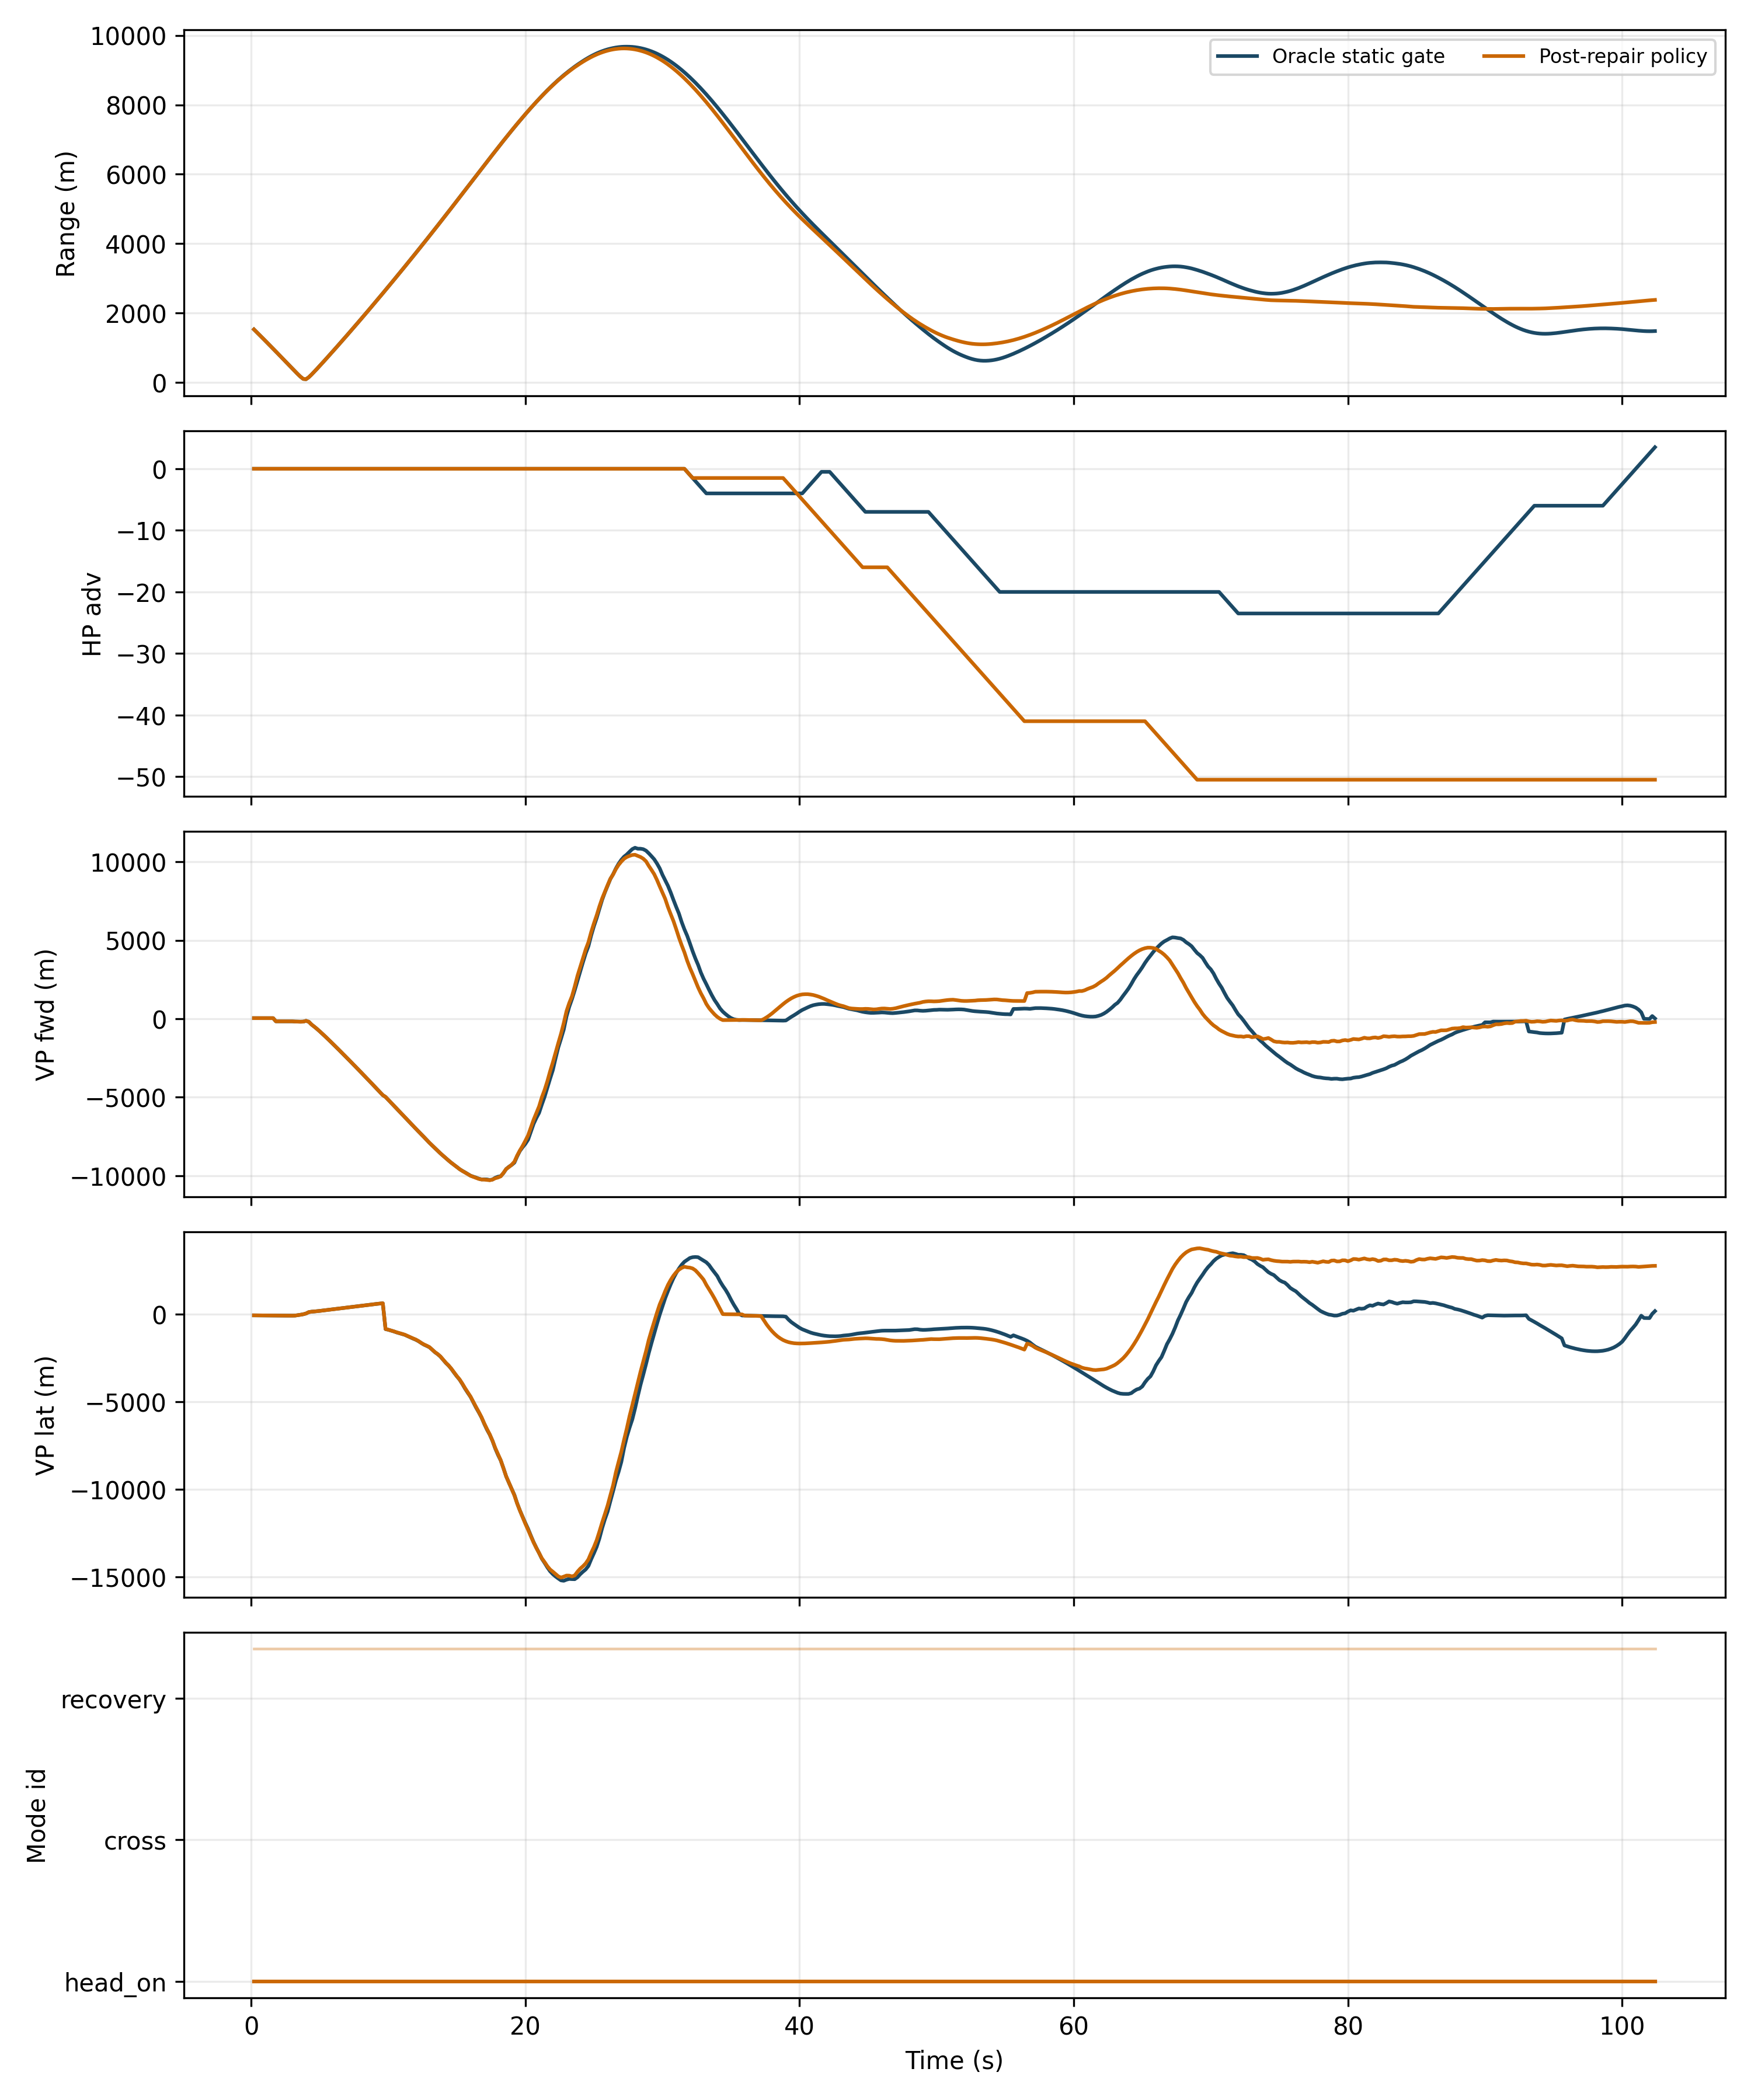
\includegraphics[width=0.85\textwidth]{figures_ast/fig2_formal_residual_r1600_timeseries_oracle_vs_recovery.png}
\caption{Residual diagnostic: expert/head\_on time series. Oracle static gate (blue) vs. post-repair policy (orange).}
\label{fig:s2}
\end{figure}

\subsection{Figure S3: Crossing evidence synthesis}

\begin{figure*}[htbp]
\centering
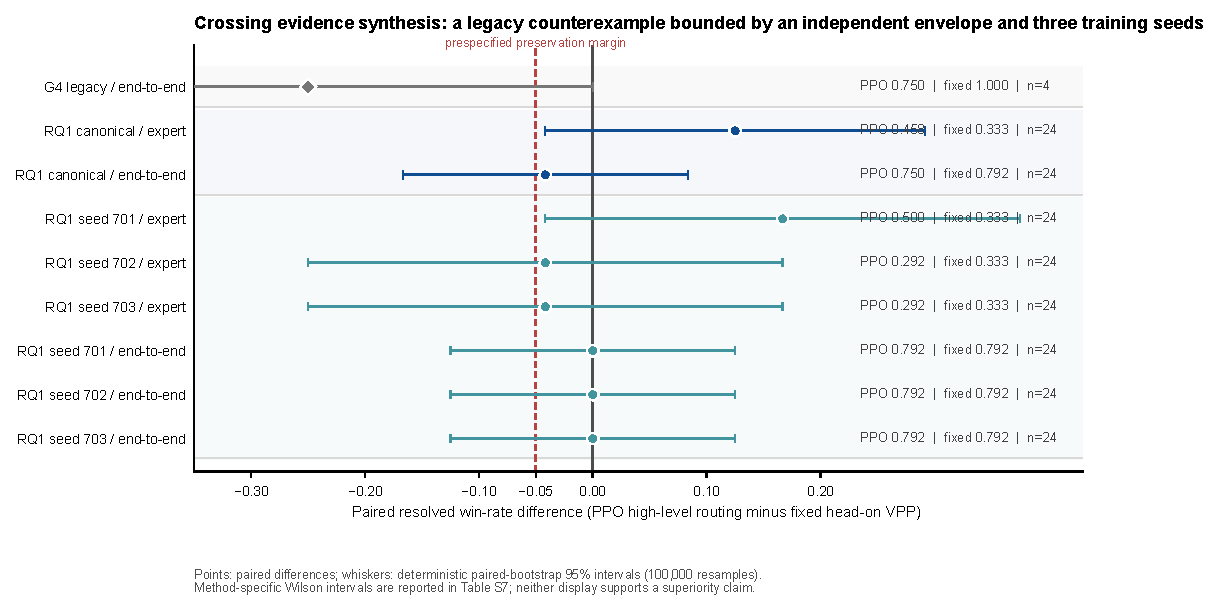
\includegraphics[width=\textwidth]{figures_ast/figure_s3_rq1_crossing_evidence_forest.pdf}
\caption{Crossing evidence synthesis. Points show paired resolved win-rate
differences (PPO high-level routing minus fixed head-on VPP); whiskers show
deterministic paired-bootstrap 95\% intervals. The dashed line denotes the
preregistered $-0.05$ practical preservation margin. The legacy G4
four-scenario counterexample is retained, while the independent 24-scenario
RQ1 envelope and three independently trained PPO seeds meet the practical
screen. Method-specific Wilson intervals and all raw counts are given in
Table~\ref{tab:crossing_evidence_synthesis}. This figure does not support a
superiority claim.}
\label{fig:rq1_crossing_evidence_forest}
\end{figure*}

\end{document}
